\section{Studio dei metodi e delle applicazioni}
In tale capitolo verranno spiegati i metodi, le applicazioni ed i concetti 
generali studiati durante la prima fase del tirocinio, accostando ad ogni 
di essi una relativa implementazione e/o utilizzo.\\
In primo luogo si troverà una definizione di serie temporale, seguita da
una spiegazione dei metodi per manipolare i dati inerenti a serie temporali 
su python, le componenti principali di una serie temporale e la loro visualizzazione
ed infine metodi per l'analisi di essi.\\
\\
Molti degli esempi forniti in questa sezione fanno riferimento a dataset disponibili
al sito ``UCI Machine Learning Repository''~\cite{dua:2019} più precisamente, come
esempio, è stato utilizzato un dataset relativo alla qualità dell'aria della città di
Beijing~\cite{dua:air_quality} (Pechino).
 
\subsection{Cos'è una serie temporale}
In statistica descrittiva, una serie storica (o temporale) si definisce come un insieme di variabili 
casuali ordinate rispetto al tempo, ed esprime la dinamica di un certo 
fenomeno nel tempo. Le serie storiche vengono studiate sia per 
interpretare un fenomeno, individuando componenti di trend, di ciclicità, 
di stagionalità e/o di accidentalità, sia per prevedere il suo 
andamento futuro~\cite{wiki:serie_storica}.
In altre parole una serie storica (o temporale) è un'insieme/serie di dati
capionati ed indicizzati nel tempo ad intervalli regolari come ore, giorni 
o anni.\\
\\
In termini più matematici: indichiamo con $\bm{Y}$ il fenomeno (ad esempio 
il prezzo della benzina dall'anno $1970$ all'anno $2010$) ed indichiamo con
$\bm{Y_t}$ un'ossevazione al tempo $\bm{t}$, con $\bm{t}$ un numero intero
compreso tra $\bm{1}$ a $\bm{T}$, dove $\bm{T}$ è il numero totale degli intervalli o 
periodi. Una serie temporale viene espressa in questa maniera 
$\bm{Y_t} = \left\{  \bm{Y_1}, \bm{Y_2}, \dots , \bm{Y_T}  \right\}$.

\begin{esempio} [\textit{Prezzo della benzina}]
    Se consideriamo come fenomeno $\bm{Y}$ il prezzo della benzina dal $1970$ al $2010$
    avremmo come numero totale di osservazioni (o numero totale di periodi) 
    $\bm{T} = \bm{40}$ dove:
    \begin{itemize}
        \setlength\itemsep{-0.5em}
        \item $\bm{Y_1}$: prezzo della benzina all'anno $1970$
        \item $\bm{Y_2}$: prezzo della benzina all'anno $1971$
        \item $\bm{Y_T} = \bm{Y_{40}}$: prezzo della benzina all'anno $2010$
    \end{itemize}

\end{esempio}


\subsection{Metodi per la gestione dei dati}
In questo sottocapitolo verranno spiegati i metodi studiati ed utilizzati per la gestione dei
dati in python, più nello specifico come caricare un dataset, una possibile rinomina delle
colonne ralative alle serie per una maggiore comprensione, individuazione dei valori
nulli ed infine una sezione relativa al filtraggio.

\paragraph{Cosa viene inteso per dataset} Per dataset si intende un insieme di
serie (nella nostra applicazione temporali) relative ad un'unica applicazione.

\begin{esempio}[\textit{Qualità dell'aria}]
    Consideriamo, per esempio, come applicazione le misurazioni di diversi parametri
    relativi alla qualità dell'aria di Genova: livello di $\mathsf{CO_2}$,
    livello di $\mathsf{SO_2}$, livello di $\mathsf{NO_2}$ e temperatura in \textdegree$\mathsf{C}$.
    In un dataset possiamo considerare ogni parametro come una serie temporale diversa ma indicizzata
    nel tempo in ugual maniera, quindi se queste misurazioni avvengono ogni ora avemo
    per ogni istante di tempo $t$ le misurazioni per ogni parametro in quell'istante.
    \begin{itemize}
        \setlength\itemsep{-0.5em}
        \item $Y_1$: livello di $\mathsf{CO_2}$, $\mathsf{SO_2}$, $\mathsf{NO_2}$ e temperatura in \textdegree$\mathsf{C}$ all'istante $1$.
        \item $Y_2$: livello di $\mathsf{CO_2}$, $\mathsf{SO_2}$, $\mathsf{NO_2}$ e temperatura in \textdegree$\mathsf{C}$ all'istante $2$.
        \item \dots
        \item $Y_T$: livello di $\mathsf{CO_2}$, $\mathsf{SO_2}$, $\mathsf{NO_2}$ e temperatura in \textdegree$\mathsf{C}$ all'istante $T$.
    \end{itemize}
    Ogni parametro in un dataset viene rappresentato come una colonna.
\end{esempio}

\subsubsection{Pacchetti utilizzati}
Per effettuare tutte le manovre relative all'elaborazione e manipolazione dei dati sono state
utilizzate funzionalità fornite da pacchetti python come \texttt{pandas} e \texttt{numpy}, essi semplificano
la scrittura di codice e velocizzano il tempo di sviluppo organizzando in maniera ottimale
i dati. Per essere utilizzati essi necessitano prima di essere installati tramite il
gestore di pacchetti di python \texttt{pip}.
\paragraph{Snippet per l'installazione dei pacchetti}
\begin{minted}{bash}
    pip install pandas
    pip install numpy
\end{minted}
\paragraph{Snippet per il caricamento in python}
\begin{minted}{python3}
    import pandas as pd
    import numpy as np
\end{minted}



\subsubsection{Caricamento di un dataset}
Per poter utilizzare i dati all'interno di python è stata utilizzata
la funzionalità di pandas \texttt{read\_csv} dove, ogni colonna fa riferimento 
ad una serie.
\paragraph{Snippet}
\begin{minted}{python3}
    dataset = pd.read_csv('data.csv')
\end{minted}





\subsubsection{Rinomina delle colonne relative alle serie}
In qualche case, il primo passo da eseguire, è quello di rinominare
le colonne relative ad ogni serie così da poter avere una rappresentazione
più accurata del dataset.
Tramite l'utilizzo della funzione \texttt{display} e del metodo \texttt{head}
del dataset possiamo controllare i primi $5$ valori di un dataset
controllando anche così il nome di ogni colonna.
\paragraph{Snippet}
\begin{minted}{python3}
    display(dataset.head())
\end{minted}
\begin{figure}[h!]
    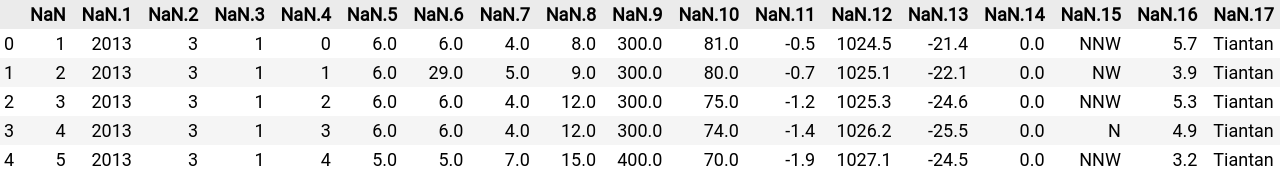
\includegraphics[width=\linewidth,height=2.7cm]{head_before_rename.png}
    \caption{output del metodo head prima della rinomina delle colonne}
    \label{fig:head_before_rename}
\end{figure}
Come si può notare nell'immagine~\ref*{fig:head_before_rename} i nomi delle colonne 
non hanno nessun nome significativo, con il seguente esempio potremmo
cambiare il nome delle colonne.

\paragraph{Snippet}
\begin{minted}{python3}
    # definizione di una lista di nomi per le colonne del dataset
    dataset.columns = [ 'no',    'year',  'month', 'day', 'hour', 
                        'pm2_5', 'pm10',  'so2',   'no2', 'co',  
                        'o3',    'temp',  'pres',  'dewp','rain',  
                        'wd',    'wspm',  'station']
    display(dataset.head())
\end{minted}
\begin{figure}[h!]
    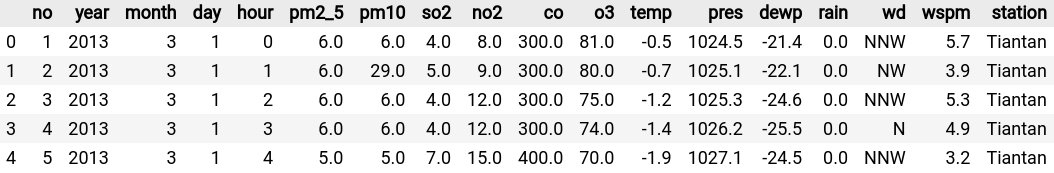
\includegraphics[width=\linewidth,height=2.7cm]{head_after_rename.png}
    \caption{output del metodo head dopo la rinomina delle colonne}
    \label{fig:head_after_rename}
\end{figure}
Come si può notare nell'immagine~\ref*{fig:head_after_rename}
assegnando la lista delle colonne come attuali nomi per le serie del dataset
riusciamo ad ottenere un'interpretazione più accurata.


\subsubsection{Scelta dell'indice}
Molte delle funzionalità fornite da \texttt{pandas} ed altri pacchetti python
richiedono che il dataset sia indicizzato nel tempo nel corretto modo.
In figura~\ref*{fig:head_after_rename} si può notare che la prima colonna
senza nome e la seconda colonna con nome \texttt{no}, indichino
il numero di riga per ogni misurazione, la differenza è che la prima colonna
è generata automaticamente dal pacchetto \texttt{pandas}, ed impostata
di default come indice, mentre la seconda con
nome \texttt{no} è fornita direttamente dal file csv precedentemente caricato.
Per l'analisi della maggior parte delle serie temporali un'idicizzazione per numero
di riga non è significativa, sarebbe molto più conveniente lavorare avendo
come indice di tabella la data ed ora di ogni effettiva misurazione.
A questo proposito il dataset caricato ci fornisce delle colonne (\texttt{year}
, \texttt{month}, \texttt{day} e \texttt{hour}) indicizzate per tempo e relative
ad ogni misurazione, che possono essere riformattate insieme ed usate come indice
per il dataset.\\
\\
\paragraph{Snippet}
\begin{minted}{python3}
    # unificazione delle colonne relative al tempo per ogni 
    # istante di tempo t in una nuova colonna
    new_index_column = []
    for i in range(len(dataset.year)):
    new_index_column.append("%s/%s/%s %s:0:0" 
        % (dataset.day[i], dataset.month[i], 
           dataset.year[i], dataset.hour[i]) )

    # elimina le colonne relative al tempo
    del dataset["year"], dataset["month"], 
        dataset["day"], dataset["hour"], 
        dataset["no"]

    # imposta/crea la nuova colonna date e converti in datetime
    dataset['date'] = new_index_column
    dataset['date'] = pd.to_datetime(dataset.date, dayfirst=True)

    # imposta come index la nuova colonna date
    dataset.set_index("date", inplace=True)
    display(dataset.head())
\end{minted}
\begin{figure}[h!]
    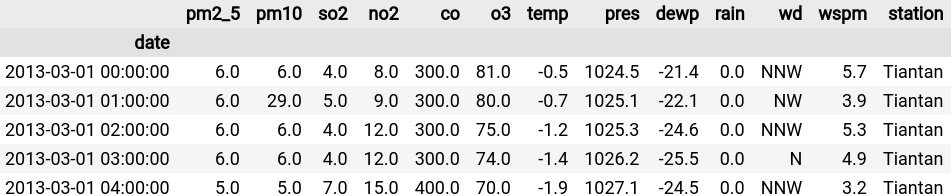
\includegraphics[width=\linewidth,height=2.7cm]{head_after_index_set.png}
    \caption{output del metodo head dopo aver impostato l'indice}
    \label{fig:head_after_index_set}
\end{figure}
Come si può notare dall'output del metodo \texttt{head} nell'immagine \ref*{fig:head_after_index_set}
\texttt{date} è stato impostato come indice di tabella e quindi da questo momento in poi
possiamo accedere al dataset, scegliendo le misurazioni interessate, utilizzando la
data.

\paragraph{Periodo di campionamento}
Un'altra importante modifica è impostare il periodo di campionamento del dataset,
in poche parole impostare un corretto indice non basta a massimizzare il corretto
funzionamento delle funzionalità di analisi delle serie temporali, bisogna anche specificare
l'istante di tempo che occorre tra una misurazione e l'altra. Per fare ciò
\texttt{pandas} fornise un metodo che imposta il periodo di campionamento
a quello deiderato, nel nostro caso sappiamo che le misurazioni sono state campionate
ogni ora.
\subparagraph{Snippet}
\begin{minted}{python3}
    # imposta il periodo di capionamento 
    # di ogni osservazione ad ogni ora
    dataset = dataset.asfreq("h")
\end{minted}

\subsubsection{Individuazione dei valori nulli e possibili soluzioni}
La presenza di valori nulli in un dataset relativo a serie temporali





% \subsubsection{Filtraggio}


